\chapter{Application Design}

\section{Description of the Chapter}
The following chapter discusses the design of the application, with regards to layout and colours used throughout each page. Within the chapter, the developer will provide wireframes with regards to the thought process of the layout resource files. The Logo of the application will also be discussed with the reason behind the naming of the application provided below.

\section{Creation of InforMe@Dublin's Logo}
The inspiration for the InforMe@Dublin came from the using Google maps location markers of which is an iconic symbol to use of which ties into the following application quite well as it utilises maps and a mobile devices real-time location. The naming of the application is as the name state's to inform someone about something which in this case is the county of Dublin. The colours of which are used in the logo were just clean and crisp looking of which complimented the other parts of the logo. Other colours that were tried just didn't tie in with the look and feel of the application.

\begin{figure}[htbp]
	\center 
\includegraphics[width=150pt]{informe}\\
	\caption{InforMe@Dublin Logo} \label{Figure: InforMe@Dublin Logo}
\end{figure}
\newpage
\section{Start Page}
While designing the startup page of the application, certain permissions are requested in order to retrieve the device's location for the application being able to use the GPS module and to access the storage of the Android phone. The following wireframe represents the application after the installation has been completed and opened the following screen will be shown to the user. While looking at the following wireframe located in figure 6.2, The logo is the first aspect of the application on which the user should see which represents what the app is actually about the layout is also smooth and well round

\par 
Looking at the wireframe which was designed by the developer the reader can see where the user may log in with their credentials as well as using OAuth sign in by linking their personal Gmail account which continues to the setup of an individual account on the InforMe@Dublin app. The button is in the lower centre of the page with the button Google sign in. With regards to the login activity, the layout is a relatively appealing design.

\begin{figure}[htbp]
    \center 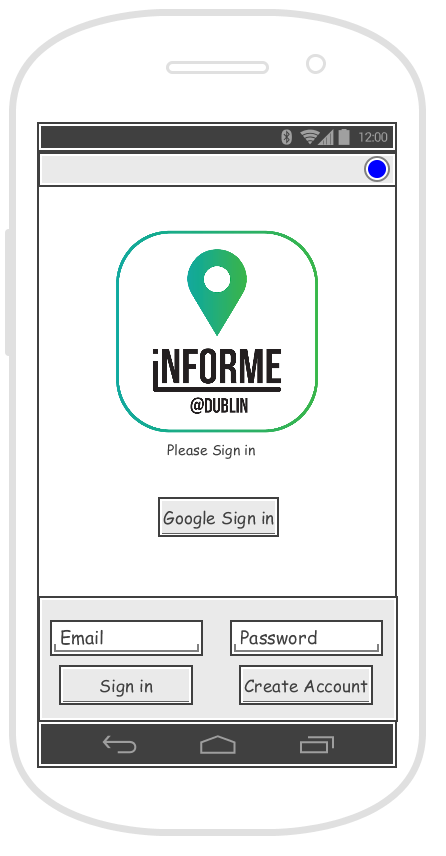
\includegraphics[width=150pt]{LoginWireframe}\\
    \caption{Login Wireframe} \label{Figure: Login Wireframe}
\end{figure}
\newpage
\section{Colour Scheme}
After looking at the first screen login wireframe. The developer would like to display the colours of which will be used throughout the app the colours are as follows. The developer chooses these specific colours as it complements the project as a whole. Are used throughout the multiple pages with are incorporated throughout the app. The following colours make for a sleek look while users are utilising the app.

\begin{enumerate}
    \item Theme of Application - R 43 / G 152 / B 212
    \item Buttons of Application - R 249 / G 159 / B 27
    \item Logo of Application - Blue: = R 0 / G 167 / B 157    Green: = 56 / G 180 / B 73 
\end{enumerate}    

\begin{figure}[htbp]
    \center 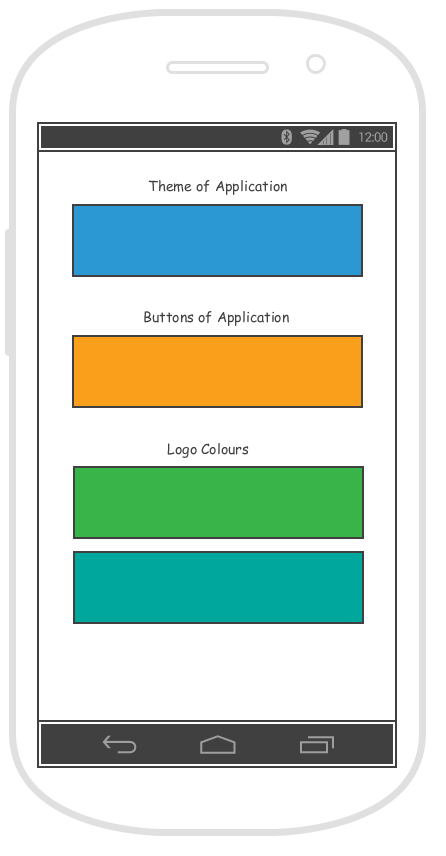
\includegraphics[width=150pt]{ColoursWireframe}\\
    \caption{Colours Wireframe} \label{Figure: Colours Wireframe}
\end{figure}

\section{Wire-frames}
The wireframes in this section of the chapter are regarding the wireframes on which were created by the developer. These wireframes were meant as a guide on how the layouts of the different activities would look like on completion of the application in question. Each styling aspect of the application was followed throughout the development. All colours used were disclosed in the above section.

\subsection{Login}
The following logged in wireframe is to be used in conjunction with the login wireframe which will authenticate the user as well as sign in the user of the application. Different display buttons will be shown to the user on authentication with both firebases authentication and the database of the Firebase API.

\begin{figure}[htbp]
    \center 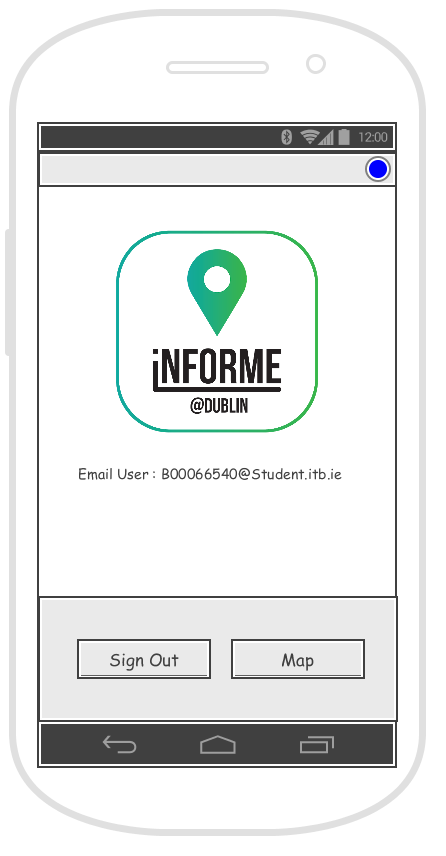
\includegraphics[width=150pt]{LoggedInWireframe}\\
    \caption{Logged in user Wireframe} \label{Figure: Logged in user Wireframe}
\end{figure}

\newpage

\subsection{Map}
With regards to the Maps Activity wireframe on which was designed by the developer, shows were the specific buttons are for the user throughout the using of the application. While viewing the wireframe, the reader can then distinguish how the real activity will be laid out. On the left-hand corner of the activity shows the compass area on which the user can choose to use. On the right-hand corner is used to toggle the focus of the user's location on which changes the camera animation to the devices current location utilising latitude and longitude. With regards to the bottom half of the screen on the bottom left-hand side of the display is where users can choose to send information to the InforMe@Dublin developer to update the Firebase database to add more historic locations for other users to enjoy.

\begin{figure}[htbp]
    \center 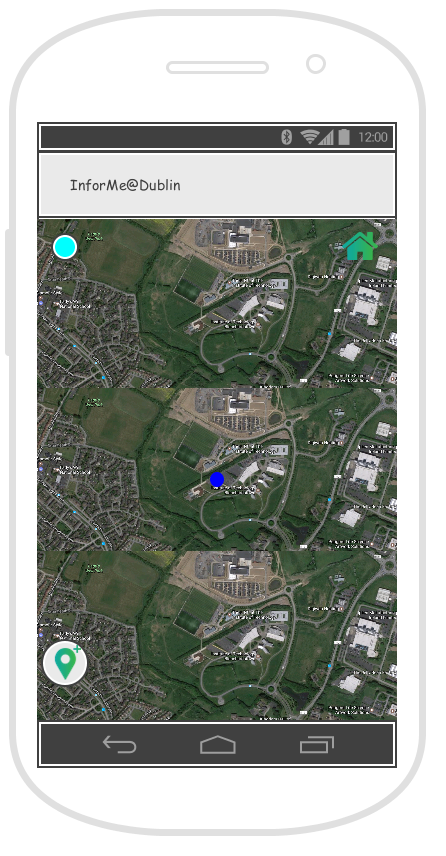
\includegraphics[width=150pt]{MapActivityWireframe}\\
    \caption{Map Activity Wireframe} \label{Figure: Map Activity Wireframe}
\end{figure}

\par
The next wireframe in this section shows what happens when the user has entered a particular geofence a dialogue is displayed with the monuments name on which the user of the application can then continue to view the information on the specific location on which the dialogue appeared for. A notification will also be sent on entering the location which is a general notification of the application notifying the user of a geofence on which they have entered.

\begin{figure}[htbp]
    \center 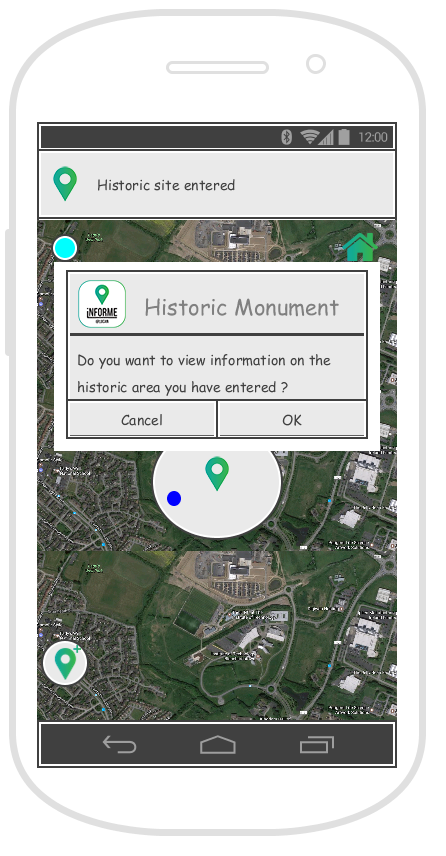
\includegraphics[width=150pt]{GeofenceMapWireframe}\\
    \caption{Map Activity Geofence Wireframe} \label{Figure: Map Activity Geofence Wireframe}
\end{figure}

\newpage
 
\subsection{Settings}
The following section of this chapter represents the settings page of the application with a more particular reference to the preferences of the application. Within the following wireframe, the following preferences can be changed in the activity that is related to the application.

\begin{figure}[htbp]
    \center 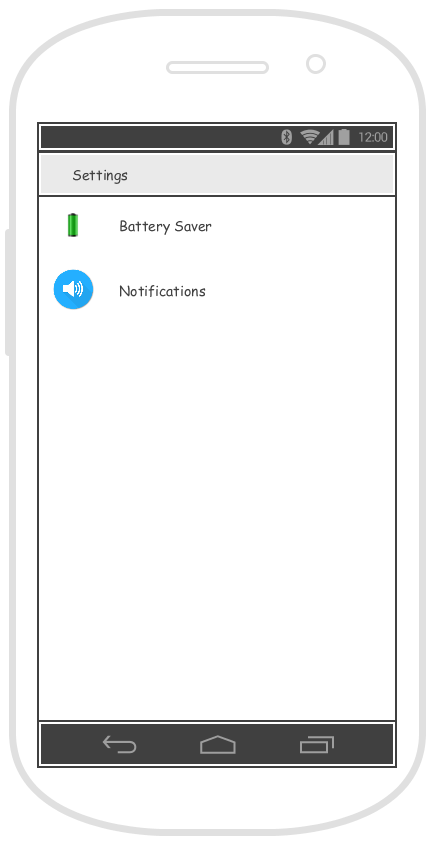
\includegraphics[width=150pt]{SettingsPreference}\\
    \caption{Settings Preferences Wireframe} \label{Figure: Settings Preferences Wireframe}
\end{figure}

\subsection{Add Information}
Concerning the following figure 6.8 shows the design on which will be implemented on the InforMe@Dublin app. with the wireframe in mind the user will be able to fill in the fields that are necessary for the app to create an email and send to the developer of the application. By pressing the select images button, the users will be brought to their personal gallery on which they can choose images to post to the developer as well as any information they might have at hand such as the location of such monuments.

\begin{figure}[htbp]
    \center 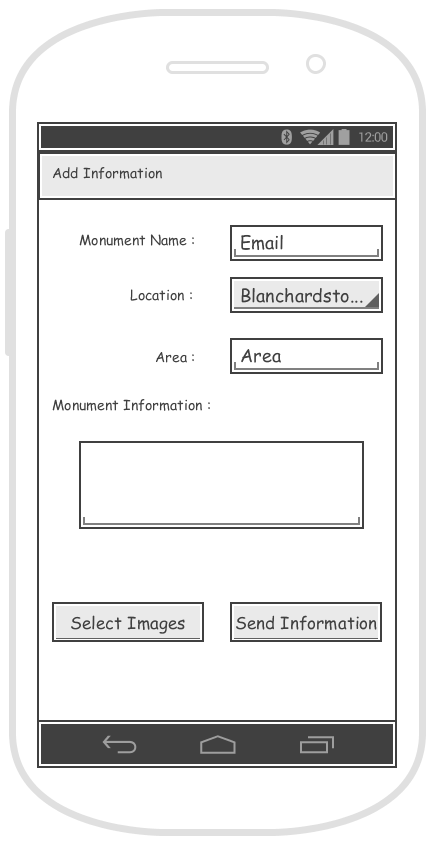
\includegraphics[width=150pt]{addInformationWireframe}\\
    \caption{Add Information Wireframe} \label{Figure: Add Information Wireframe}
\end{figure}


\subsection{Show Information}
With relation to the following section located in the system design. Two wireframes were developed in which the developer of the application could get a better understanding of what he wanted to achieve. The following wireframes were turned into resource layout files to complete the look and feel, and the developer thought that these following layout files would be the most important design in such an application. Information is the most important factor in the project which needs to be portrayed to the user in a specific manner. Creating a crisp clean and non-cluttered layout was the key ingredient which why the wireframes layout below was chosen.
\par
While looking at both figures 6.9 and 6.10, the reader can see the distinctive feel of what the developer is trying to achieve by using both of the following activity wireframes as fragments the developer can create a smooth turn around feel of the information on which the users want to see. While looking at figure 6.9, users can get to grasp with the images that have been used from multiple sources. The information that the reader can see is just filler text that was generated from a website. Were the filler text is in the wireframe is compiled of the information from that monument which was sourced from multiple sources on the internet. A button which is shown as a loudspeaker icon will then perform a text-to-speech on the information which was retrieved from the Firebase database.

\begin{figure}[!tbp]
    \centering
    \begin{minipage}[b]{0.4\textwidth}
        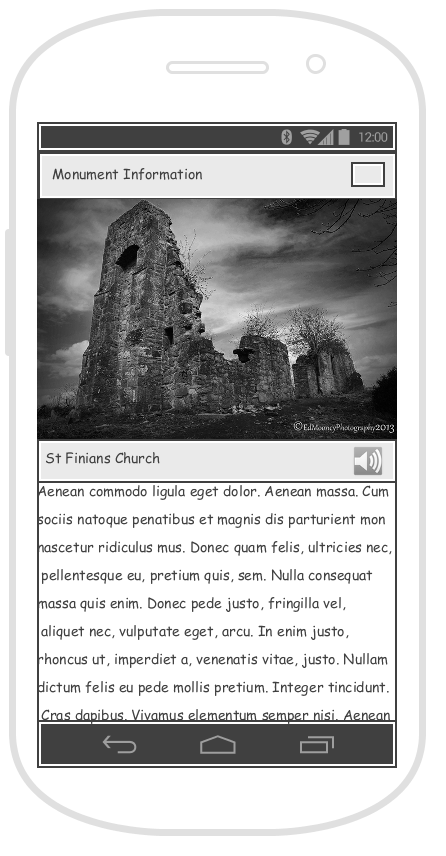
\includegraphics[width=\textwidth]{DisplayInformationWireframe}
        \caption{Display Information }
        \label{Figure: Display Information }
    \end{minipage}
    \hfill
    \begin{minipage}[b]{0.4\textwidth}
        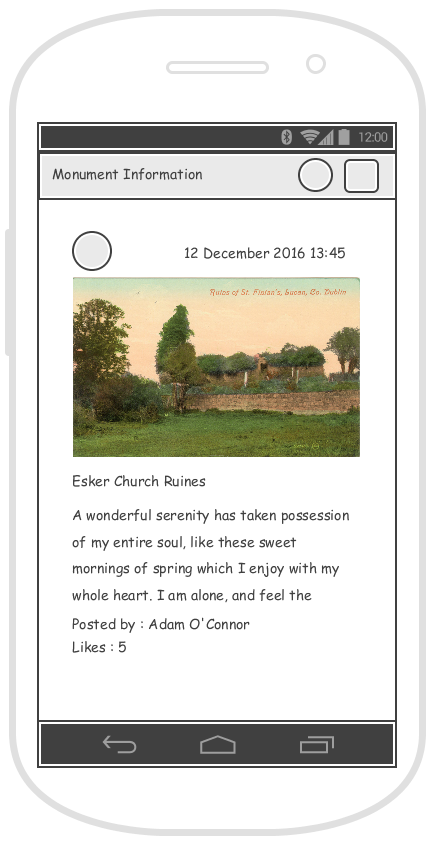
\includegraphics[width=\textwidth]{ViewPostsWireframe}
        \caption{View Posts } 
        \label{Figure: View Posts }
    \end{minipage}
\end{figure}

\section{Summary of the Chapter}
To conclude the chapter as a whole, the reader can see that the developer has discussed the design of the InforMe@Dublin application. Each page of the app has been mocked up which allowed the developer to visualise how it should look at the end of development. While providing these wireframes in this current chapter, the reader can grasp a much better understanding of how the application prototype will evolve throughout the time of development and also with regards to the time scale allowed on which the final build and release of the project will be of the date 27th of April. The next chapter in this thesis discusses the coding of the application on the loading of geofences, providing permissions to the user on Android Marshmallow OS and above and many more feature on which were incorporated into the app. Each separate part of the next chapter will be discussed with regards to the different methods of which are associated with its specific method. 